\section{Rivers \& Streams}

KELLEY ET AL. --> Terrain simulation using a model of stream erosion

TERRAIN ADAPTED TO RIVERS

In the work by Kelly et al. the user specifies, on a horizontal plane, the terrain outline along with the main trunk stream. The terrain outline is used to configure the terrain extremities once ported to a 3 dimensional space. The main trunk stream specifies the path which the highest order water stream should follow on the resulting terrain.\\
Given the terrain outline and the position of the initial main trunk stream, the system calculates the drainage area the stream is responsible for. If this value surpasses a preconfigured constant, the stream will be split to form new streams, each channelling a smaller drainage area. This constant depends on the type of soil as resistant materials (e.g. stone) will be stronger and less susceptible to splitting than weaker ones (e.g. clay). This splitting process is repeated iteratively until a balance is found where each stream is able to channel their associated drainage area. After which a plausible elevation is calculated for each stream junction and, subsequently, a plausible terrain generated.\\


Derzapf ET AL. --> RIVER NETWORKS FOR INSTANT PROCEDURAL PLANETS

TERRAIN ADAPTS TO RIVER

In their work, Derzapf et al. permit the creation of procedural planets at any scale in real-time. To do so, only a rough representation of the planet is generated and detailed content is produced on-the-fly when the user navigates through it. This has the advantage of keeping memory usage minimum whilst not compromising on realism. To ensure updates are performed in real-time, their algorithms are implemented to take use of the massively parallel architecture of GPUs. \\
To initialise high-level planets, the system first creates the base mesh with all contained vertices representing the sea. The system then selects a given number of seed continent vertices and allows them to spread until a user-configured land-to-water ratio is reached. At this point, the "rough" planet is a mesh with each vertex assigned one of two labels: continent or sea.\\
To create the rivers the system iterates through all continental vertices in pseudo-random order to find those that are adjacent to a sea vertex. When such a vertex is found, it acts as the river mouth from which adjacent continental vertices chosen pseudo-randomly are connected. This is performed iteratively to form the river networks.\\
To assign ground altitudes to the river vertices the system employs the following formula for each river vertex, starting from the river mouth:

$a_{v} = a_{u} + e_{a}l_{e}\xi , e_{a} = \frac{a_{max_river}}{l_{r}} $

Where:
\begin{itemize}
\item $a_{v}$ is the ground altitude of the current vertex.
\item $a_{u}$ is the ground altitude of the previously processed vertex (or zero if \textit{v} is the first vertex).
\item $e_{a}$ is the average ground elevation.
\item $l_{e}$ is the length of the current vertex.
\item $\xi \in [0,1[$ is a uniformly distributed pseudo-random number.
\item $a_{max_river}$ is the user-configured maximum river altitude.
\item $l_{r}$ is the current river length.
\end{itemize}

When the ground altitudes have been assigned, the following formula is used iteratively on each river vertex to assign water altitudes:

$w_{v} = a_{v} + e_{w}l_{e}, e_{w} = \frac{\epsilon_{river}}{l_{cr}} $

Where:
\begin{itemize}
\item $w_{v}$ is the water altitude of the current vertex.
\item $a_{v}$ is the ground altitude of the current vertex.
\item $e_{w}$ is the average water elevation.
\item $l_{e}$ is the length of the current vertex.
\item $\epsilon_{river}$ is the maximum river depth.
\item $l_{cr}$ is the distance from the current vertex to the river spring.
\end{itemize}

Once this has been performed, the "rough terrain" is comprised of continental vertices, river vertices and sea vertices, each with a defined altitude.\\

All randomness in the algorithms depends on a configured seed value, enabling virtual virtual worlds to be easily reproducible. This has the added advantage of permitting networked users to explore the same virtual world with very little data exchange. \\


SMELIK ET AL. --> INTERACTIVE CREATION OF VIRTUAL WORLDS USING PROCEDURAL SKETCHING

RIVER ADAPTS TO TERRAIN, EXPLICIT USER CONTROL

In their work, Smelik et al. create an interactive system which permits users to model a complete virtual world with content ranging from rural features (mountains, rivers, etc.) to man-made ones (buildings, road networks). In order to promote user-intuitiveness, they focus strongly on user controls and develop novel interaction tools which include sketch recognition.\\
When modelling the virtual world, interactions are split into two modes: \textbf{Landscape} and \textbf{Feature}. \textit{Landscape mode} permits the designer to paint ecotopes onto the terrain using traditional image editing tools. These ecotopes are predefined by the user and encompass both elevation and soil material information. In \textit{feature mode}, the user is able to place terrain content which include rivers. To place these rivers, the user must sketch vector lines outlining the core path of the river. Based on this information, a suitable course is plotted through the landscape, river banks inserted and other terrain features to which the river takes precedence adapted. For example, if the river is plotted to pass through a forest, trees on the rived bed and bank will be removed. 


Pmsinkiewicz ET AL. --> A fractal model of mountains and rivers

TERRAIN ADAPTS TO RIVER

In their work, Pmsinkiewicz et al. use an adapted midpoint-displacement technique to procedurally generate plausible rivers on terrain. Midpoint-displacement is a fractal technique heavily used for the creation of realistic looking terrain height-maps. Given a starting triangle representing the terrain, \textit{A}, midpoint-displacement iteratively subdivides \textit{A} into four smaller triangles. Each time new triangle vertices are created they are displaced vertically by a random offset. This process is repeated until a given recursion limit is reached. See figure \ref{Midpoint displacement} for an example of a single iteration of the process.

\begin{figure}[h]
  \centering
	\label{Midpoint displacement}
	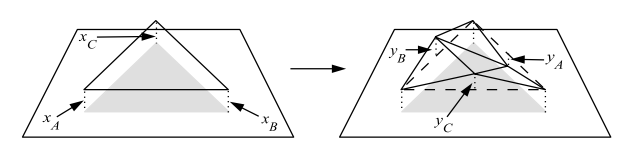
\includegraphics[width=\textwidth]{midpoint_displacement.png}
	\caption{A single iteration of midpoint displacement for the creation of mountains \cite{Prusinkiewicz1993}. New vertices $y_{A}$, $y_{B}$ and $y_{C}$ are created and shifted vertically by a random offset}
\end{figure}

To adapt this method to the generation of rivers on the terrain, the edges of each newly formed triangle are labelled as \textit{entry}, \textit{exit} or \textit{neutral}. An entry edge defines the point of entry for the river into the triangle, an exit edge the point of exit and a neutral edge prevents the river from passing through.\\

When a production step is applied and a triangle split, the following constraints must be applied:
\begin{itemize}
\item An entry edge must split into an entry and a neutral edge.
\item An exit edge must split into an exit edge and a neutral edge.
\item A neutral edge must split into two neutral edges.
\item The newly formed edge-pairs within the triangle must either be "entry/exit" or "neutral/neutral".
\end{itemize}

See figure \ref{Single production of midpoint displacement adapted to river generation. Given the initial triangle, four valid split scenarios. } for example valid productions.

\begin{figure}[h]
  \centering
	\label{Single production of midpoint displacement adapted to river generation. Given the initial triangle, four valid split scenarios. }
	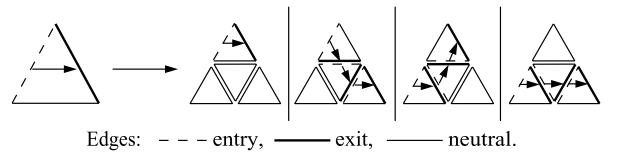
\includegraphics[width=\textwidth]{midpoint_displacement_for_rivers_1.png}
	\caption{Single production of midpoint displacement adapted to river generation \cite{Prusinkiewicz1993}. Given the initial triangle, four valid split scenarios.}
\end{figure}

One difficulty with this technique is to ensure two adjacent triangles are coherent once they split. That is, that the exit edge of one coincides with the entry edge of the other edge. To overcome this, the location of the vertices of an edge are used as the key to a random number generating hash table which, depending on its output, determines which segment will be crossed by the river.\\
When complete, a river path which is guaranteed not to cross itself is created. Post-processing is then used to create realistic terrain surrounding the riverbed.

Belhadj et Audibert --> Modeling landscapes with ridges and rivers: bottom up approach

RIVER ADAPTED TO TERRAIN

In their work Belhadg et Audibert \cite{Belhadj2005} automate the creation of ridges and river networks on the terrain. To create the ridges, particle pairs are first placed at random locations on the terrain. These particle pairs are then randomly assigned an axis and, iteratively, both particles distance themselves in opposite directions, perpendicular to this axis. At each iteration, a new height is calculated for the vertex. The heights decrease with distance from the start point following a Gaussian distribution.\\
To create the river networks, river particles are placed on the top of the newly generated ridges and a simple physical simulation is used to model the motion of these particles on the terrain. The path followed by these particles are tracked and, when two paths intersect, their particle velocity and mass are combined. When all particles have stopped moving the simulation is deemed balances and all particle paths which do not lead to terrain extremities are discarded. The remaining particle paths are kept and form the river network. To initialise the remaining vertices on the terrain, interpolation is performed based on the height of its surrounding river and ridge vertices.


